En este proyecto el soporte matemático tiene una importancia destacada. Es por ello que se han tenido que superar retos como: el movimiento de los motores de forma coordinada para alcanzar
diversas posiciones a lo largo del rango de movilidad del brazo.

La relación entre los ángulos de los ejes y el punto final del brazo no es trivial y 
es necesario un estudio previo de distintos factores para poder hacerlo correctamente. 
Por una parte, es necesario definir de la manera más precisa posible la configuración 
geométrica del brazo. Dicha configuración relaciona los distintos segmentos que
conforman el manipulador según una convención de parámetros
que trabaja sobre las posibles articulaciones que componen el brazo robótico 
y que se denotan por $Z_i$, donde $i$ es el número de la articulación.

En particular, las relaciones a estudiar son:

\begin{itemize}
    \item El ángulo presente entre dos articulaciones adyacentes
          $\widehat{Z_aZ_b}~rad$, el cual se denota por `$\alpha_b$'.
    \item La distancia presente entre dos articulaciones adyacentes
          $\overline{Z_aZ_b}$, representada por `$a_b$'.
    \item El sentido de la rotación de una articulación,
          $\overrightarrow{X_aY_a}$, denotada por `$\theta_a$'.
\end{itemize}

Estas relaciones permiten establecer la configuración geométrica del robot,
fundamental para poder definir los movimientos posibles del mismo y generar tanto
las matrices de la cinemática directa como obtener las ecuaciones de la cinemática
inversa. Además, se puede obtener de la misma manera las matrices Jacobianas que
permiten conseguir datos útiles como el trabajo, la velocidad o la potencia.

Para el $\mu$Arm, se obtuvieron las siguientes configuraciones geométricas:

\begin{figure}[H]
    \centering
    \begin{minipage}{.4\linewidth}
        \centering
        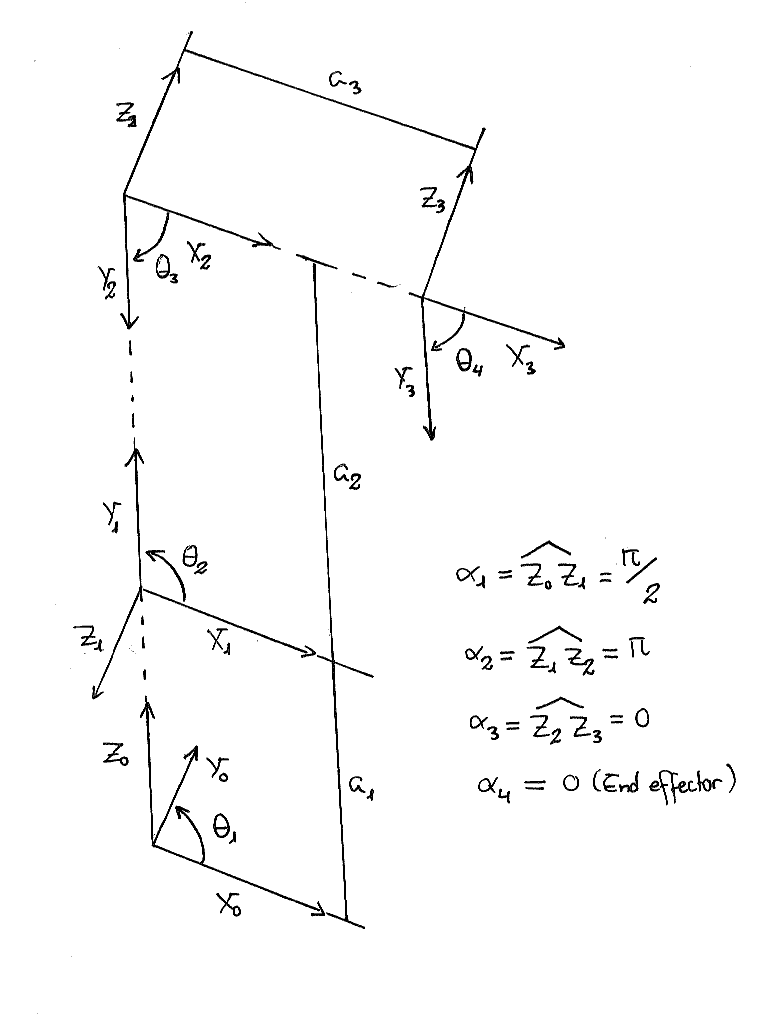
\includegraphics[width=\textwidth]{pictures/geometric_configuration_2.png}
        \caption{Configuración geométrica del $\mu$Arm.}
        \label{fig:uArm_gc}
    \end{minipage}
    \hfill
    \begin{minipage}{.48\linewidth}
        \centering
        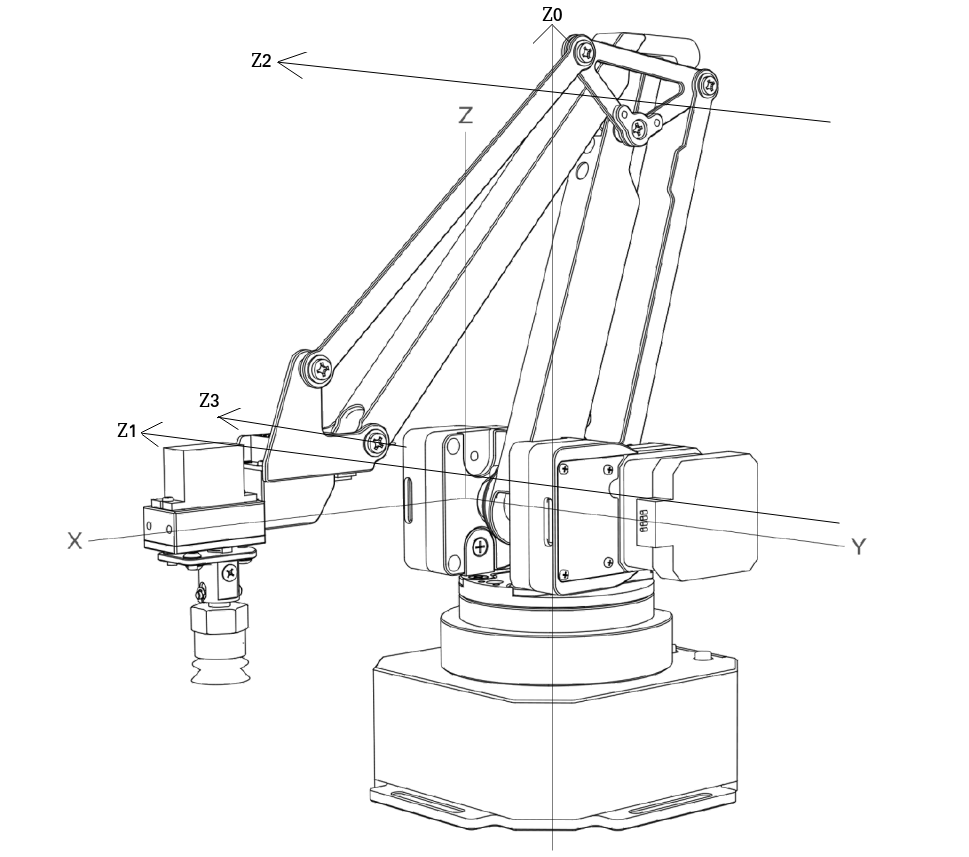
\includegraphics[width=\textwidth]{pictures/axis.png}
        \caption{Los distintos grados de libertad del $\mu$Arm, representados por $Z_i$.}
        \label{fig:uArm_axis}
    \end{minipage}
\end{figure}

Con estos valores, ya se pueden obtener las distancias entre articulaciones así
como las desviaciones entre las mismas, si las hay. En el caso particular del $\mu$Arm,
se obtiene unos datos como los siguientes (las medidas se han obtenido desde la guía del
desarrollador de UFACTORY\cite{ufactoryUArmSwiftPro2017}):

\begin{table}[ht]
    \begin{minipage}{.49\linewidth}
        \begin{figure}[H]
            \centering
            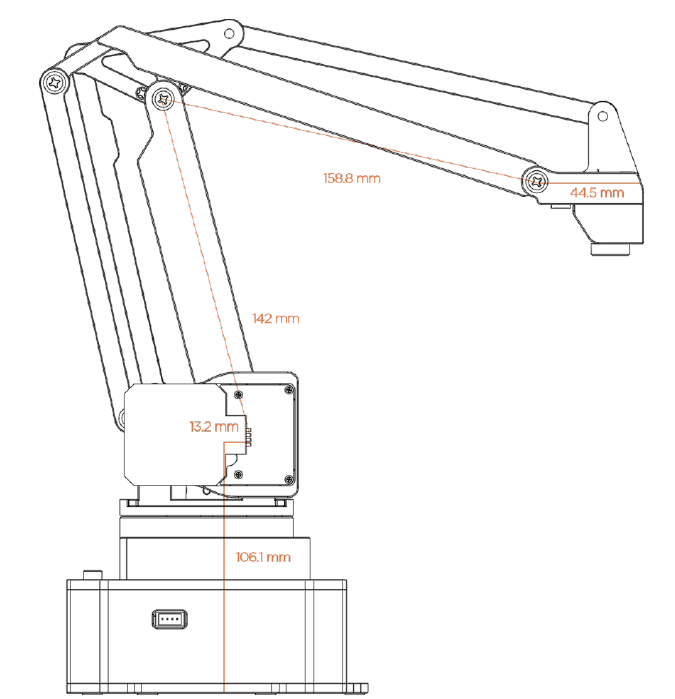
\includegraphics[width=\linewidth]{pictures/sizes.png}
            \caption{Longitudes del brazo robótico \cite{ufactoryUArmSwiftPro2017}.}
            \label{fig:sizes}
        \end{figure}
    \end{minipage}
    \hfill
    \begin{minipage}{.49\linewidth}
        \centering
        \begin{tabular}{|| c | c c ||}
            \hline
            $i$ & $a_i~(mm.)$ & $d_i~(mm.)$ \\ [0.5ex]
            \hline\hline
            $1$ & $13.2$      & $106.1$     \\
            \hline
            $2$ & $142$       & $0$         \\
            \hline
            $3$ & $158.8$     & $0$         \\
            \hline
            $4$ & $44.5$      & $0$         \\ [1ex]
            \hline
        \end{tabular}
        \caption{Longitudes y desviaciones del manipulador $\mu$Arm.}
        \label{tab:uArm-ld-values}
    \end{minipage}
\end{table}

Esta información permite construir una tabla de \textit{Denavit--Hartenberg} que
recoge la información del robot. Dicha tabla se conoce también como ``parámetros de
\textit{Denavit--Hartenberg}'', que conforman cuatro variables que recogen, en una
convención particular, la referencia de una cadena cinemática (objetos rígidos unidos
a articulaciones que responden a una función matemática) o de un brazo robótico \cite{DenavitHartenbergParameters2020}.

La convención de parámetros de \textit{Denavit--Hartenberg} son los siguientes:
\begin{itemize}
    \item $d_i$ -- distancia desde el origen de coordenadas de $Z_{i - 1}$ a la normal común\footnote{la normal
              común de dos articulaciones que no intersecan se define como la línea perpendicular a
              ambos ejes, que se usa para conocer la distancia entre ambos \cite{CommonNormalRobotics2017}.}
          con $Z_i$.
    \item $\theta_i$ -- el ángulo de rotación que forman el eje $X_{i - 1}$ y el eje $X_i$,
                    tomando como eje de rotación $Z_{i - 1}$. El sentido del ángulo viene definido además
                    por $x_i$ hasta $y_i$.
    \item $a_i$ -- la distancia de los ejes $Z_i$ y $Z_{i - 1}$, medida sobre su normal común $\left(\overline{Z_iZ_{i-1}}\right)$.
    \item $\alpha_i$ -- el ángulo, tomando como eje de rotación la normal común, desde $Z_{i - 1}$ hacia $Z_i$ $\left(\widehat{Z_aZ_b}\right)$.
\end{itemize}

Esta convención es especialmente interesante porque permite definir de forma precisa
las relaciones entre las articulaciones, pudiendo conocer la rotación relativa entre
dos de ellas y la traslación entre sus puntos. Además, aplicando las propiedades
de las matrices, se puede obtener la relación absoluta entre las rotaciones y las
traslaciones, lo que se traduce en conocer el punto exacto $\left\{x, y, z\right\}$ en el que se encuentra el
\textit{end--effector} cuando se giran las articulaciones
$\left\{\theta_0, \theta_1, \cdots, \theta_i\right\}~rad$ respectivamente.

Esta relación se representa mediante una matriz, definida en la ecuación \ref{eq:dh-matrix}:

\begin{equation}
    \label{eq:dh-matrix}
    {
    \displaystyle \operatorname {}
    ^{i-1}T_{i}=\left[{
                \begin{array}{ccc|c}
                    \cos{\theta_{i}} & -\sin{\theta_{i}}\cos{\alpha_{i}} & \sin{\theta_{i}}\sin{\alpha_{i}}  & a_{i}\cos{\theta_{i}} \\
                    \sin{\theta_{i}} & \cos{\theta_{i}}\cos{\alpha_{i}}  & -\cos{\theta_{i}}\sin{\alpha_{i}} & a_{i}\sin{\theta_{i}} \\
                    0                & \sin{\alpha_{i}}                  & \cos{\alpha_{i}}                  & d_{i}                 \\
                    \hline
                    0                & 0                                 & 0                                 & 1
                \end{array}}\right] =
    \left[{
                \begin{array}{ccc|c}
                      &   &   &   \\
                      & R' &   & T' \\
                      &   &   &   \\
                    \hline
                    0 & 0 & 0 & 1
                \end{array}}
        \right]
    }
\end{equation}

donde $R'$ representa la \textit{rotación relativa} y $T'$ la \textit{traslación relativa}.

Otra ventaja de los parámetros de \textit{Denavit--Hartenberg} es la posibilidad de
definir elementos cinemáticos\footnotemark[2], como la velocidad $\left(W_{i,j}(k)\right)$ y la aceleración ($H_{i,j}(k)$)
de distintos cuerpos así como elementos dinámicos tales como la inercia $\left(J\right)$,
el momento lineal y angular $\left(\Gamma\right)$ o las fuerzas y torques aplicados
$\left(\Phi\right)$ \footnote{si bien estos datos resultan muy útiles, para el proyecto no se consideran
    necesariamente relevantes, ya que están supeditados a la velocidad y a la masa (cuanto mayores sean,
    la aplicación de dichos elementos cinemáticos será mayor sobre los componentes del
    manipulador), y el brazo robótico no presenta ni una masa suficientemente elevada ni alcanza velocidades altas
    como para afectar en gran media al comportamiento del mismo, pero sí se contempla realizar un estudio para completar
    este proyecto en una futura versión.}.

Para un manipulador basado estructuralmente en el $\mu$Arm, se obtienen unos parámetros
de \textit{Denavit--Hartenberg} como los mostrados en la tabla \ref{tab:dh-params-with-phi}:

\begin{table}[H]
    \centering
    \begin{tabular}{ c | c c c c }
        $i$ & $\theta_i$ & $d_i~(mm.)$ & $a_i~(mm.)$ & $\alpha_i$          \\ [0.5ex]
        \hline
        $1$ & $\theta_1$ & $d_1$       & $a_1$       & $\nicefrac{\pi}{2}$ \\
        $2$ & $\theta_2$ & $0$         & $a_2$       & $\pi$               \\
        $3$ & $\theta_3$ & $0$         & $a_3$       & $0$                 \\
        $4$ & $\theta_4$ & $0$         & $a_4$       & $0$                 \\ [1ex]
    \end{tabular}
    \caption{Tabla inicial de \textit{Denavit–Hartenberg} para un manipulador basado en el $\mu$Arm parametrizada.}
    \label{tab:dh-params-with-phi}
\end{table}

Además, también se vio que este tipo de estructuras pantográficas
tienen su \textit{end--effector} siempre paralelo al plano del suelo (equivalente
a que el ángulo con el plano $X$ es $\phi_e = \pi$), por lo que el cuarto elemento de
los parámetros de \textit{Denavit--Hartenberg} para un manipulador basado en el $\mu$Arm
se puede obviar para luego añadirlo como una traslación en el eje $Z$ $\left(T_Z\right)$,
quedando como se muestra en la tabla \ref{tab:dh-params}:

\begin{table}[H]
    \centering
    \begin{tabular}{ c | c c c c }
        $i$ & $\theta_i$ & $d_i~(mm.)$ & $a_i~(mm.)$ & $\alpha_i$          \\ [0.5ex]
        \hline
        $1$ & $\theta_1$ & $d_1$       & $a_1$       & $\nicefrac{\pi}{2}$ \\
        $2$ & $\theta_2$ & $0$         & $a_2$       & $\pi$               \\
        $3$ & $\theta_3$ & $0$         & $a_3$       & $0$                 \\ [1ex]
    \end{tabular}
    \caption{Tabla de \textit{Denavit–Hartenberg} para un manipulador basado en el $\mu$Arm parametrizada.}
    \label{tab:dh-params}
\end{table}

Esta característica simplifica los cálculos del ángulo final ya que siempre es el mismo
$\left(\pi~rad\right)$, quedando únicamente por calcular los valores de $\theta_2$ y 
$\theta_3$.

Una vez obtenidos los datos correspondientes al robot, podemos definir múltiples 
relaciones entre los mismos:
\begin{itemize}
    \item La cinemática directa, la cual permite saber el punto $\left\{x, y, z\right\}$
          según unos ángulos $\left\{\theta_0, \theta_1, \theta_2\right\}$ de entrada.
    \item La cinemática inversa, que permite conocer qué ángulos 
          $\left\{\theta_0, \theta_1, \theta_2\right\}$ posicionan el robot en un punto
          $\left\{x, y, z\right\}$.
    \item La matriz Jacobiana, donde se puede obtener un movimiento $\overrightarrow{x}$ según 
          qué velocidad haya en las articulaciones $\overrightarrow{q}$.
    \item La matriz Jacobiana inversa, la cual devuelve el valor de la velocidad en
          las articulaciones $\overrightarrow{q}$ para generar un movimiento en el 
          \textit{end--effector} $\overrightarrow{x}$.
\end{itemize}

Dado que las cuatro relaciones anteriores son útiles para conocer y definir
el comportamiento del robot, se estudiarán todas ellas para ver cómo se pueden utilizar
en el manipulador.